\subsection{Guía de Uso}

	\subsubsection{Uso general de la aplicación}
		
		\begin{figure}[hp]
		\centering
		\hspace*{-0.9in}
		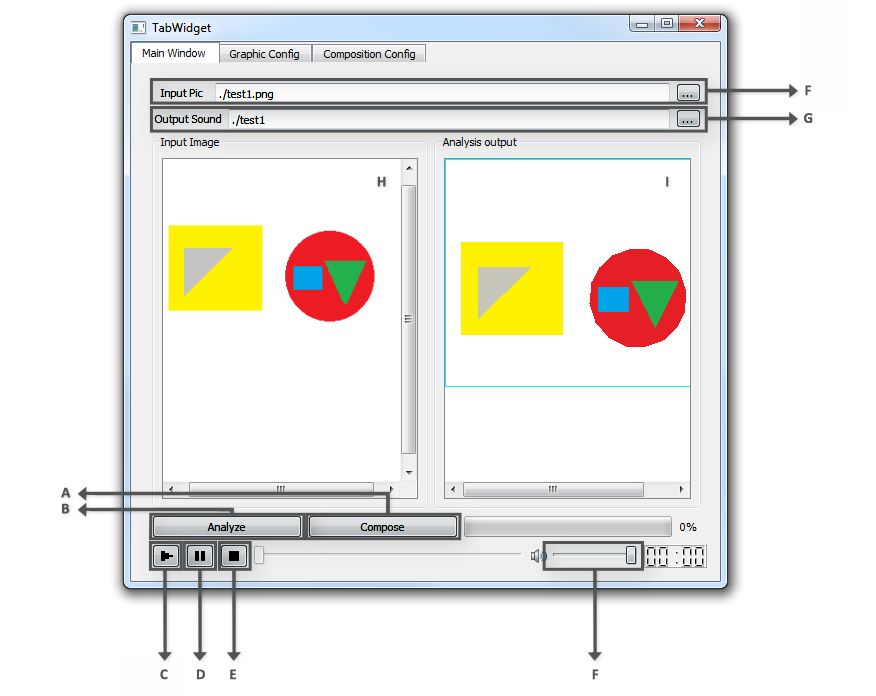
\includegraphics[scale=0.57]{graphics/interfaz.png}
		\caption{Vista general de la aplicación}
		\label{fig:interfaz}
		\end{figure}

		\vspace{0.2in}\noindent\textbf{Main Window:}
		\vspace{0.2in}\\Esta pestaña se encarga de la interacción directa con el usuario, muestra los resultados obtenidos y permite lanzar los distintos componentes de la aplicación. 
		\\Esta compuesta por los siguientes elementos tal y como se puede ver en la imagen adjunta:\\
		
		\noindent\textit{Carga de imagen de entrada [Botón 6]:}  Mediante esta opción el usuario puede elegir la dirección desde donde se cargará la imagen de entrada que se usará en el análisis. Para elegir la dirección podrá insertar el texto a mano o utilizar el botón para usar el explorador del sistema operativo correspondiente.\\
		
		\noindent\textit{Selección del archivo de audio de salida [Botón 7]:}  Mediante esta opción el usuario puede la dirección dodne se guardará el archivo de salida. Para elegir la dirección podrá insertar el texto a mano o utilizar el botón para usar el explorador del sistema operativo correspondiente.\\
		
		\noindent\textit{Input Image [Panel A]:} En este panel se muestra la imagen elegida para el análisis.\\
		
		\noindent\textit{Analysis output [PANEL B]:} En este panel se muestra el resultado del último análisis realizado pulsando el botón "Analyze".\\
		
		\noindent\textit{Botón Analyze [Botón 2]:} Tal y como su nombre indica, Analyze, realiza el analisis de la imagen pasada como parámetro de entrada lanzando a ejecución el programa Phic, uno de los módulos de la aplicación. Tras analizarse, el resultado podrá observarse en el \textit{[PANEL A]}.\\
		
		\noindent\textit{Botón Compose:} Realiza la composición musical a partir de los datos analizados, para ello lanza a ejecución el programa Mu, otro de los módulos de la aplicación. Una vez compuesta la pieza musical, se podrá escuchar mediante los controles de control de sonido.\\
		
		\textit{Botones del reproductor:} Estas herramientas estan comunicadas con la librería Phonon que se encarga de la interacción con el archivo de audio creado, y una vez compuesta la melodía tomarán el parametro de entrada como referencia y cuando el usuario pulse los distintos botones realizara las distintas funciones de play, pause, stop, cambiar el volumen, o moverse a lo largo de la melodía.\\


   uso general de la aplicaicon

   uso de configuraciones graficas

   uso de configuraciones de sonido

   

          troubleshooting - librerias y demas
		  
